\begin{figure}[htp]
	\begin{center}
	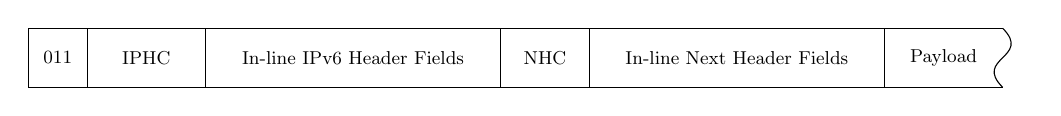
\begin{tikzpicture}[scale=0.75, every node/.append style={scale=0.75}]
		\draw (0,0) -- ++(16.5,0);
		\draw (0,1) -- ++(16.5,0);
		\draw (0,0) -- ++(0,1);
		\draw (16.5,0) .. controls (16,0.5) and (17,0.5) .. (16.5,1);

		\draw (1,0) -- ++(0,1);
		\node at (0.5, 0.5) {\small 011};

		\draw (3,0) -- ++(0,1);
		\node at (2, 0.5) {\small IPHC};

		\draw (8,0) -- ++(0,1);
		\node at (5.5, 0.5) {\small In-line IPv6 Header Fields};

		\draw (9.5,0) -- ++(0,1);
		\node at (8.75, 0.5) {\small NHC};

		\draw (14.5,0) -- ++(0,1);
		\node at (12, 0.5) {\small In-line Next Header Fields};

		\node at (15.5, 0.5) {\small Payload};
	\end{tikzpicture}
	\end{center}
	\caption{IPHC Frame Format}
	\label{fig:6lo_iphc_frame}
\end{figure}